\chapter{Key Management Entity}
\label{ch:kme}%
In the previous chapter, we summarized the history of the key exchange problem. Then, we pointed out Quantum Key Distribution as the solution to the problem. Following the fundamental laws of quantum mechanics, QKD can offer information-theoretic security. In this way, all the computational concerns that affect classical key-exchange algorithms such as Diffie-Hellman are avoided.

A secret sequence of bits produced by a couple of devices exploiting QKD cannot have a fixed length decided a priori, as explained in \ref{ch1:length}. However, the applications that want to exploit the secret key for encrypting a communication require the key to have a fixed length, usually a power of 2. For example, the Advanced Encryption Standard (AES) \cite{aes}, the most widely-used symmetric encryption algorithm, exploits keys of 128, 192, or 256 bits only.

Here we introduce the Key Management Entity (KME), the application managing the creation of fixed-length keys. We will see that this is not the only duty of the KME, and we will analyze all of them in detail.

Before diving into the KME, we formalize the concepts of Quantum Channel and Secure Application Entity. Hence, we focus on the distinction between sequences of bits produced by a Quantum Channel - which we call \textit{blocks} - and sequences of bits produced by the KME, denoted as \textit{keys}.

The following section analyzes the interaction between KME and the applications based on the standard ETSI GS QKD 014, described in detail. Then, the communication between KME and Quantum Channel is analyzed. In the end, the interaction between all the actors is explored in order to provide a complete overview of the system.

\section{Actors: KME, SAE and QC}
Here we introduce the leading entities of the quantum key distribution system we will describe.

First of all, a pair of devices able to build sequences of bits exploiting QKD protocols is called \textbf{Quantum Channel (QC)}. Each device is a QKD Entity (QKDE). The way a Quantum Channel produces sequences of bits has been described in the first chapter.

Each QKD Entity is linked to a \textbf{Key Management Entity (KME)}. The KME is the entity that manages keys in the network in cooperation with one or more other Key Management Entities.

Applications requesting one or more keys from a Key Management Entity are called \textbf{Secure Application Entities (SAE)}. In particular, the SAEs asking for the generation of new keys are called "master SAEs"; the ones asking for keys associated with given IDs are called "slave SAEs".

\section{Keys and blocks}
\label{kme:keys_vs_blocks}

We will distinguish "keys" and "blocks" from now on.

The product of a Quantum Channel is called \textbf{block}. A Universally Unique Identifier (UUID) \cite{uuid} identifies a block and contains a sequence of bits produced exploiting Quantum Key Distribution protocols: the \textit{block material}. Once again, it is essential to underline that the block material has a length that cannot be established a priori.

Instead, the product of a Key Management Entity will be called \textbf{key}. A UUID also identifies a key. It contains a sequence of bits, often referred to as \textit{key material}. However, the length of the key material can be determined by the KME. We will see that a key is built exploiting bits of one or more blocks.

The figure below quickly shows the leading entities of the network and what kind of information they exchange. QCs provide blocks to KMEs, while KMEs provide keys to SAEs.

\begin{figure}[H]
    \centering
    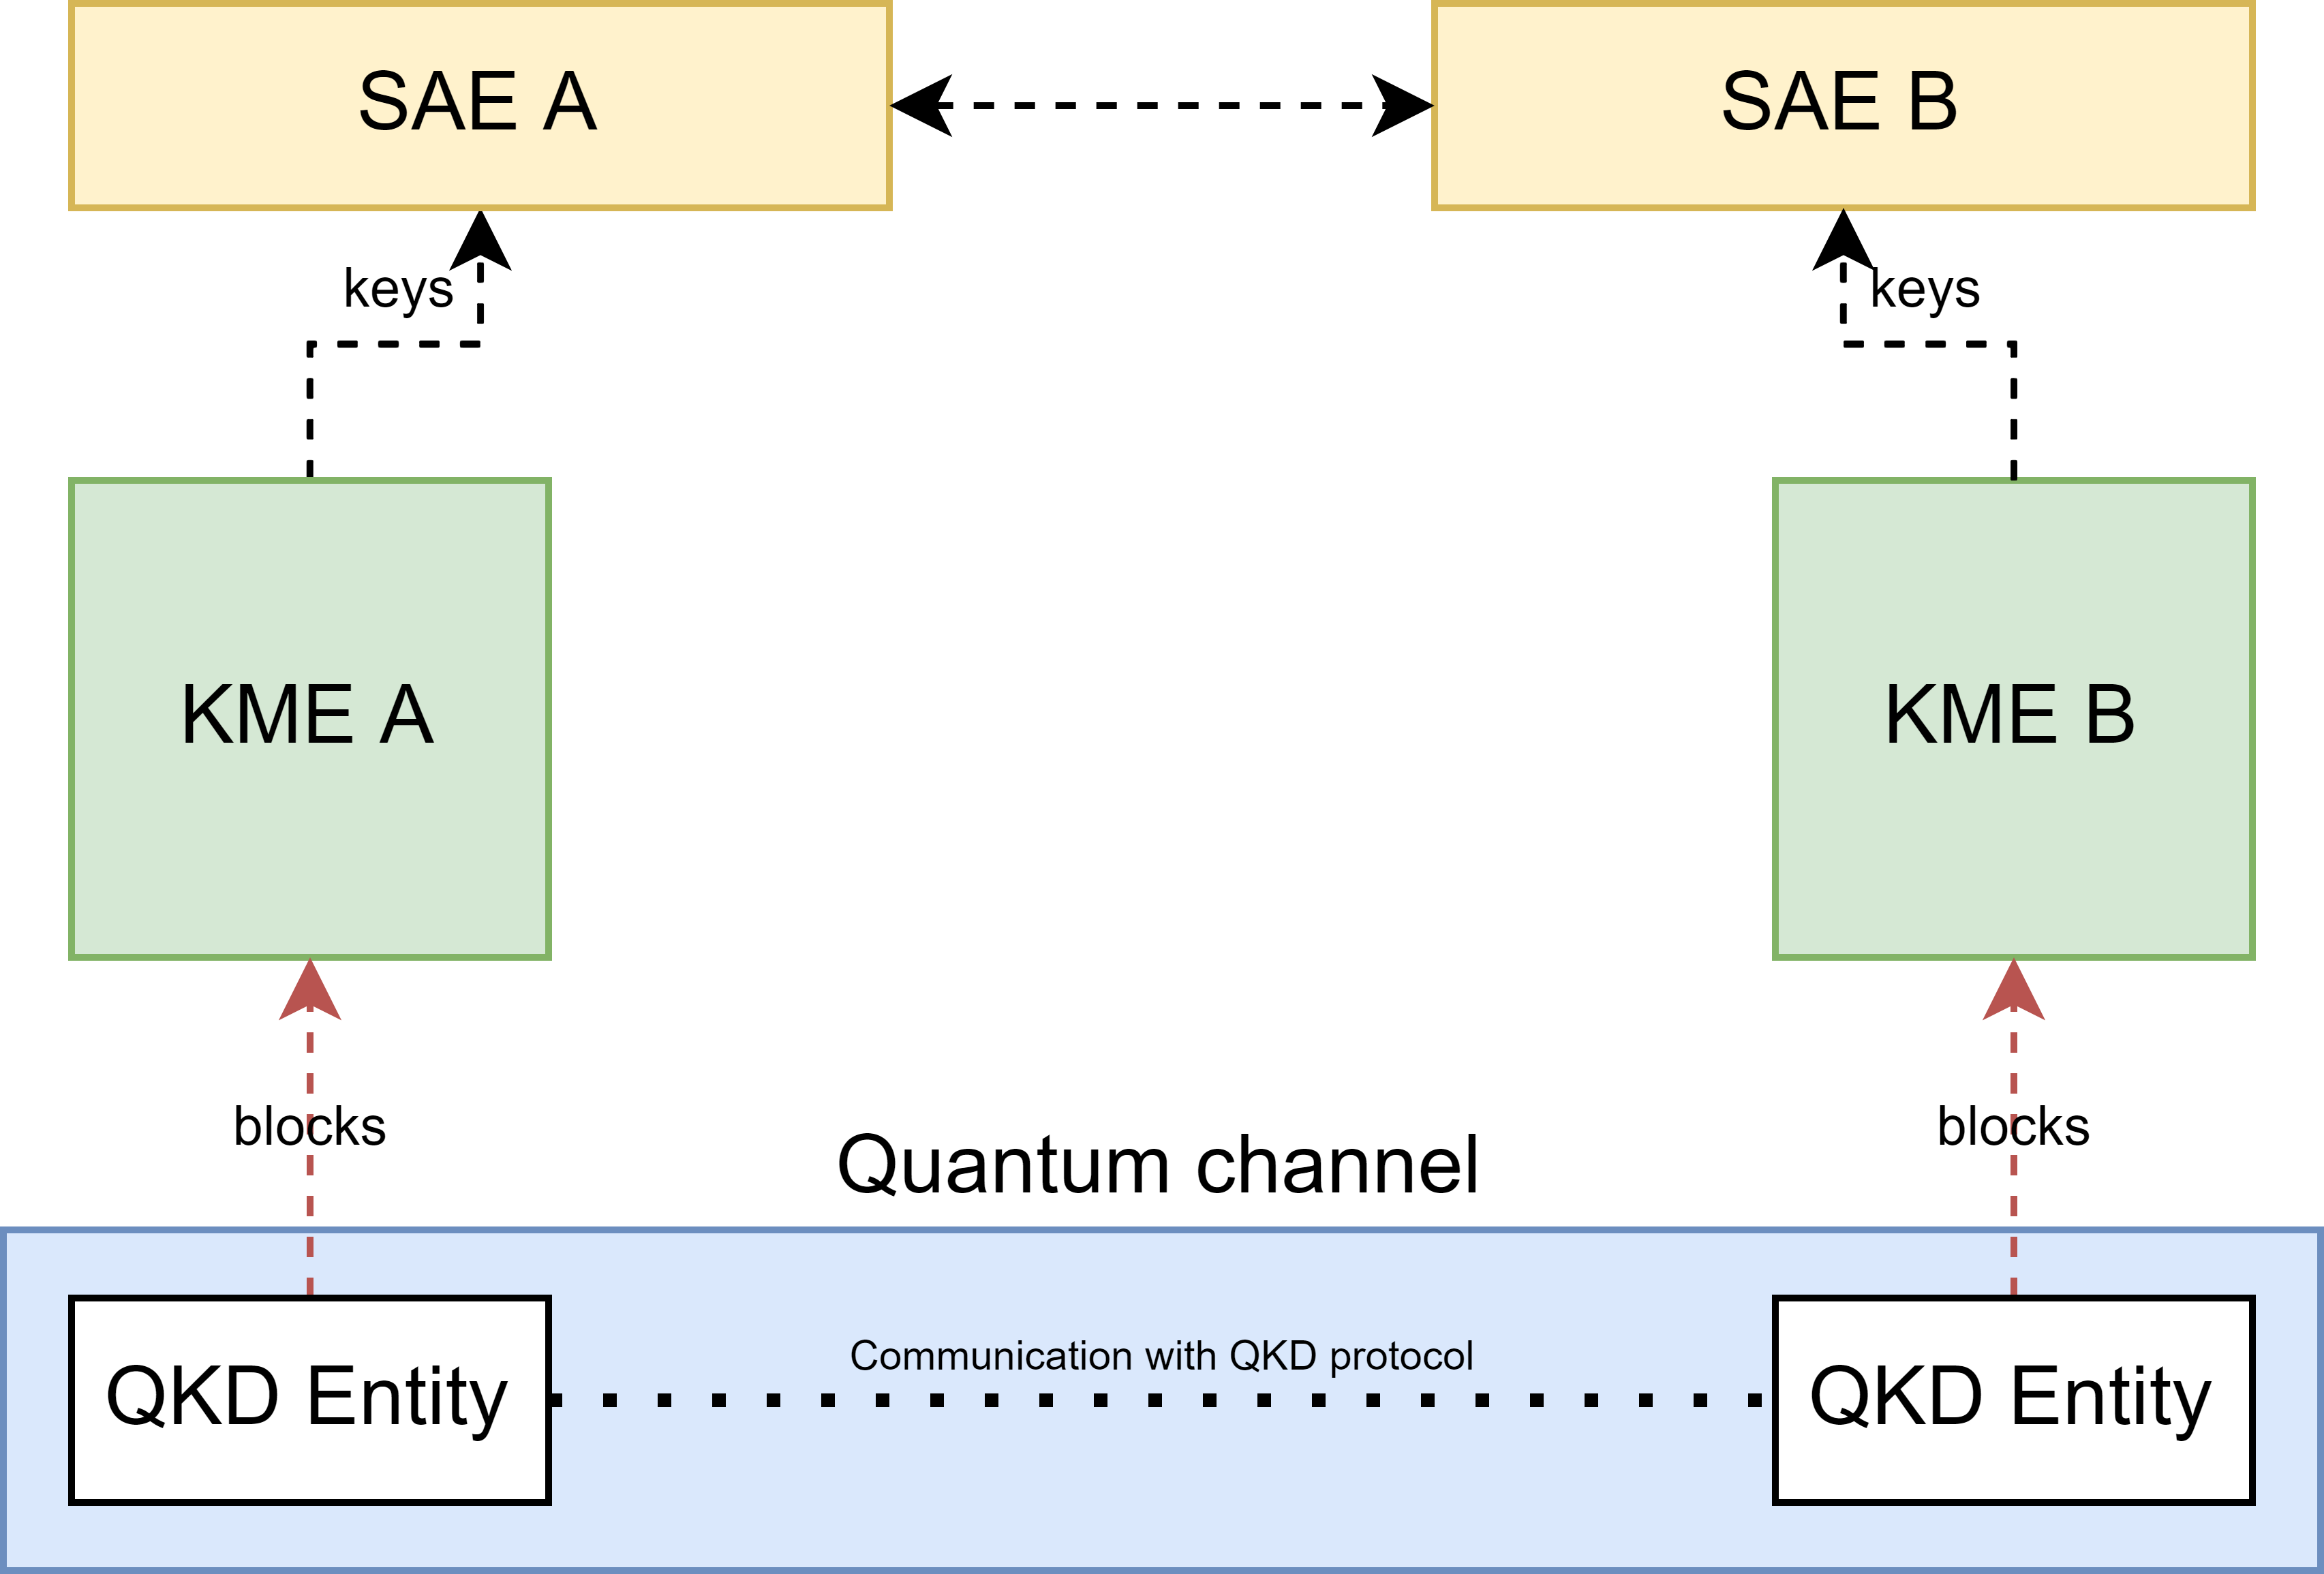
\includegraphics[width=0.8\textwidth]{overview}
    \caption{An overview of the network.}
    \label{fig:overview}
\end{figure}

\section{The interaction between the KME and the SAE}
This section will focus on the interaction between a Key Management Entity and one or more Secure Application Entities. The interface between these two entities has been implemented following standard ETSI GS QKD 014 \cite{etsi014}.

The standard ETSI GS QKD 014 defines an Application Programming Interface (API) that SAEs can exploit to send requests to KMEs. Each request is made through the HTTP protocol \cite{http}, the most widely-used protocol for internet communication. Data in the message body of HTTP requests from SAE to KME and HTTP responses from KME to SAE are encoded in JSON format \cite{json}.

In particular, an application may request:
\begin{itemize}
    \item the generation of one or more new keys
    \item the keys associated with one or more given key IDs
    \item the status of the KME (e.g., how many keys the KME can produce for each request, the maximum length of a produced key...)
\end{itemize}

There is an interface defined by the standard mentioned above for each of these three requests.

In the following sub-sections, we will dive into the specification of each interface.

\subsection{Generating keys}

\subsubsection{Key generation request}
\label{kme:key_gen}

A SAE that needs the generation of N keys of equal size S may use the HTTP GET method \textit{/enc\_keys}, specifying the "number" and the "size" as request parameters.

For example, if a SAE wants two keys of length 256, it may send an HTTP GET request with the following path:
\mint{latex}{/enc_keys?number=2&size=256}

There may be situations where the SAE wants to communicate some extra information to the KME. In this case, the SAE may exploit the HTTP POST method \textit{/enc\_keys}. Instead of specifying the "number" and "size" parameters, the HTTP POST method has a body whose data format is defined as a Key Request JSON data format. The Key Request JSON data format looks like this:

\usemintedstyle{borland}
\begin{minted}{json}
{
    "number": 2,
    "size": 256,
    "extension_mandatory": [
        { "abc_route_type": "direct" },
        { "abc_transfer_method": "qkd" }
    ],
    "extension_optional": [
        { "abc_max_age": 30000 }
    ]
}
\end{minted}

The "number" and "size" fields have the same meanings as the corresponding URL parameters.

"extension\_mandatory" is an array of name/value pairs representing extension parameters. The KME shall handle them or return an error.

"extension\_optional" is also an array of extensions specified as name/value pairs, but the KME may ignore these.

For more details on the Key Request JSON data format, see page 15 of the standard mentioned above.

\subsubsection{Key generation response}
\label{kme:key_container}
Despite the HTTP request received, the KME tries to generate the requested number of keys. How the KME produces keys will be discussed in the following sections. If the KME can produce the requested number of keys with the needed length and respect the mandatory extensions, its HTTP response will have a body containing a Key Container JSON data format. The following is an example of a Key Container JSON data format:

\begin{minted}{json}
{
  "keys": [
    {
      "key_ID": "ed4a8b14-0f5e-44c3-a28c-46e3df35dda4",
      "key": "jj86XIbUR9LVRVJaqoxcgw9mBaVzQHBtc8JEh9DUgAA="
    },
    {
      "key_ID": "23e0dfa1-e6f8-4477-a2c8-c7b0f9684769",
      "key": "aYXpqHpBgtH0rd7qubqTpSQ36fCReDeG6MBWPhkD/LI="
    }
  ]
}
\end{minted}

The Key Container is an array of keys. For each key, the UUID and the key material are given. Notice that the standard defines the key material field as "key". The key material is encoded as a base64 string \cite{base64}. Base64 is a binary-to-text encoding scheme designed to carry data stored in binary formats across channels that only reliably support text content.

For more details on the Key Container JSON data format, see pages 16-17 of the standard mentioned above.

Here is an example overview of a successful key generation request:
\begin{figure}[H]
    \centering
    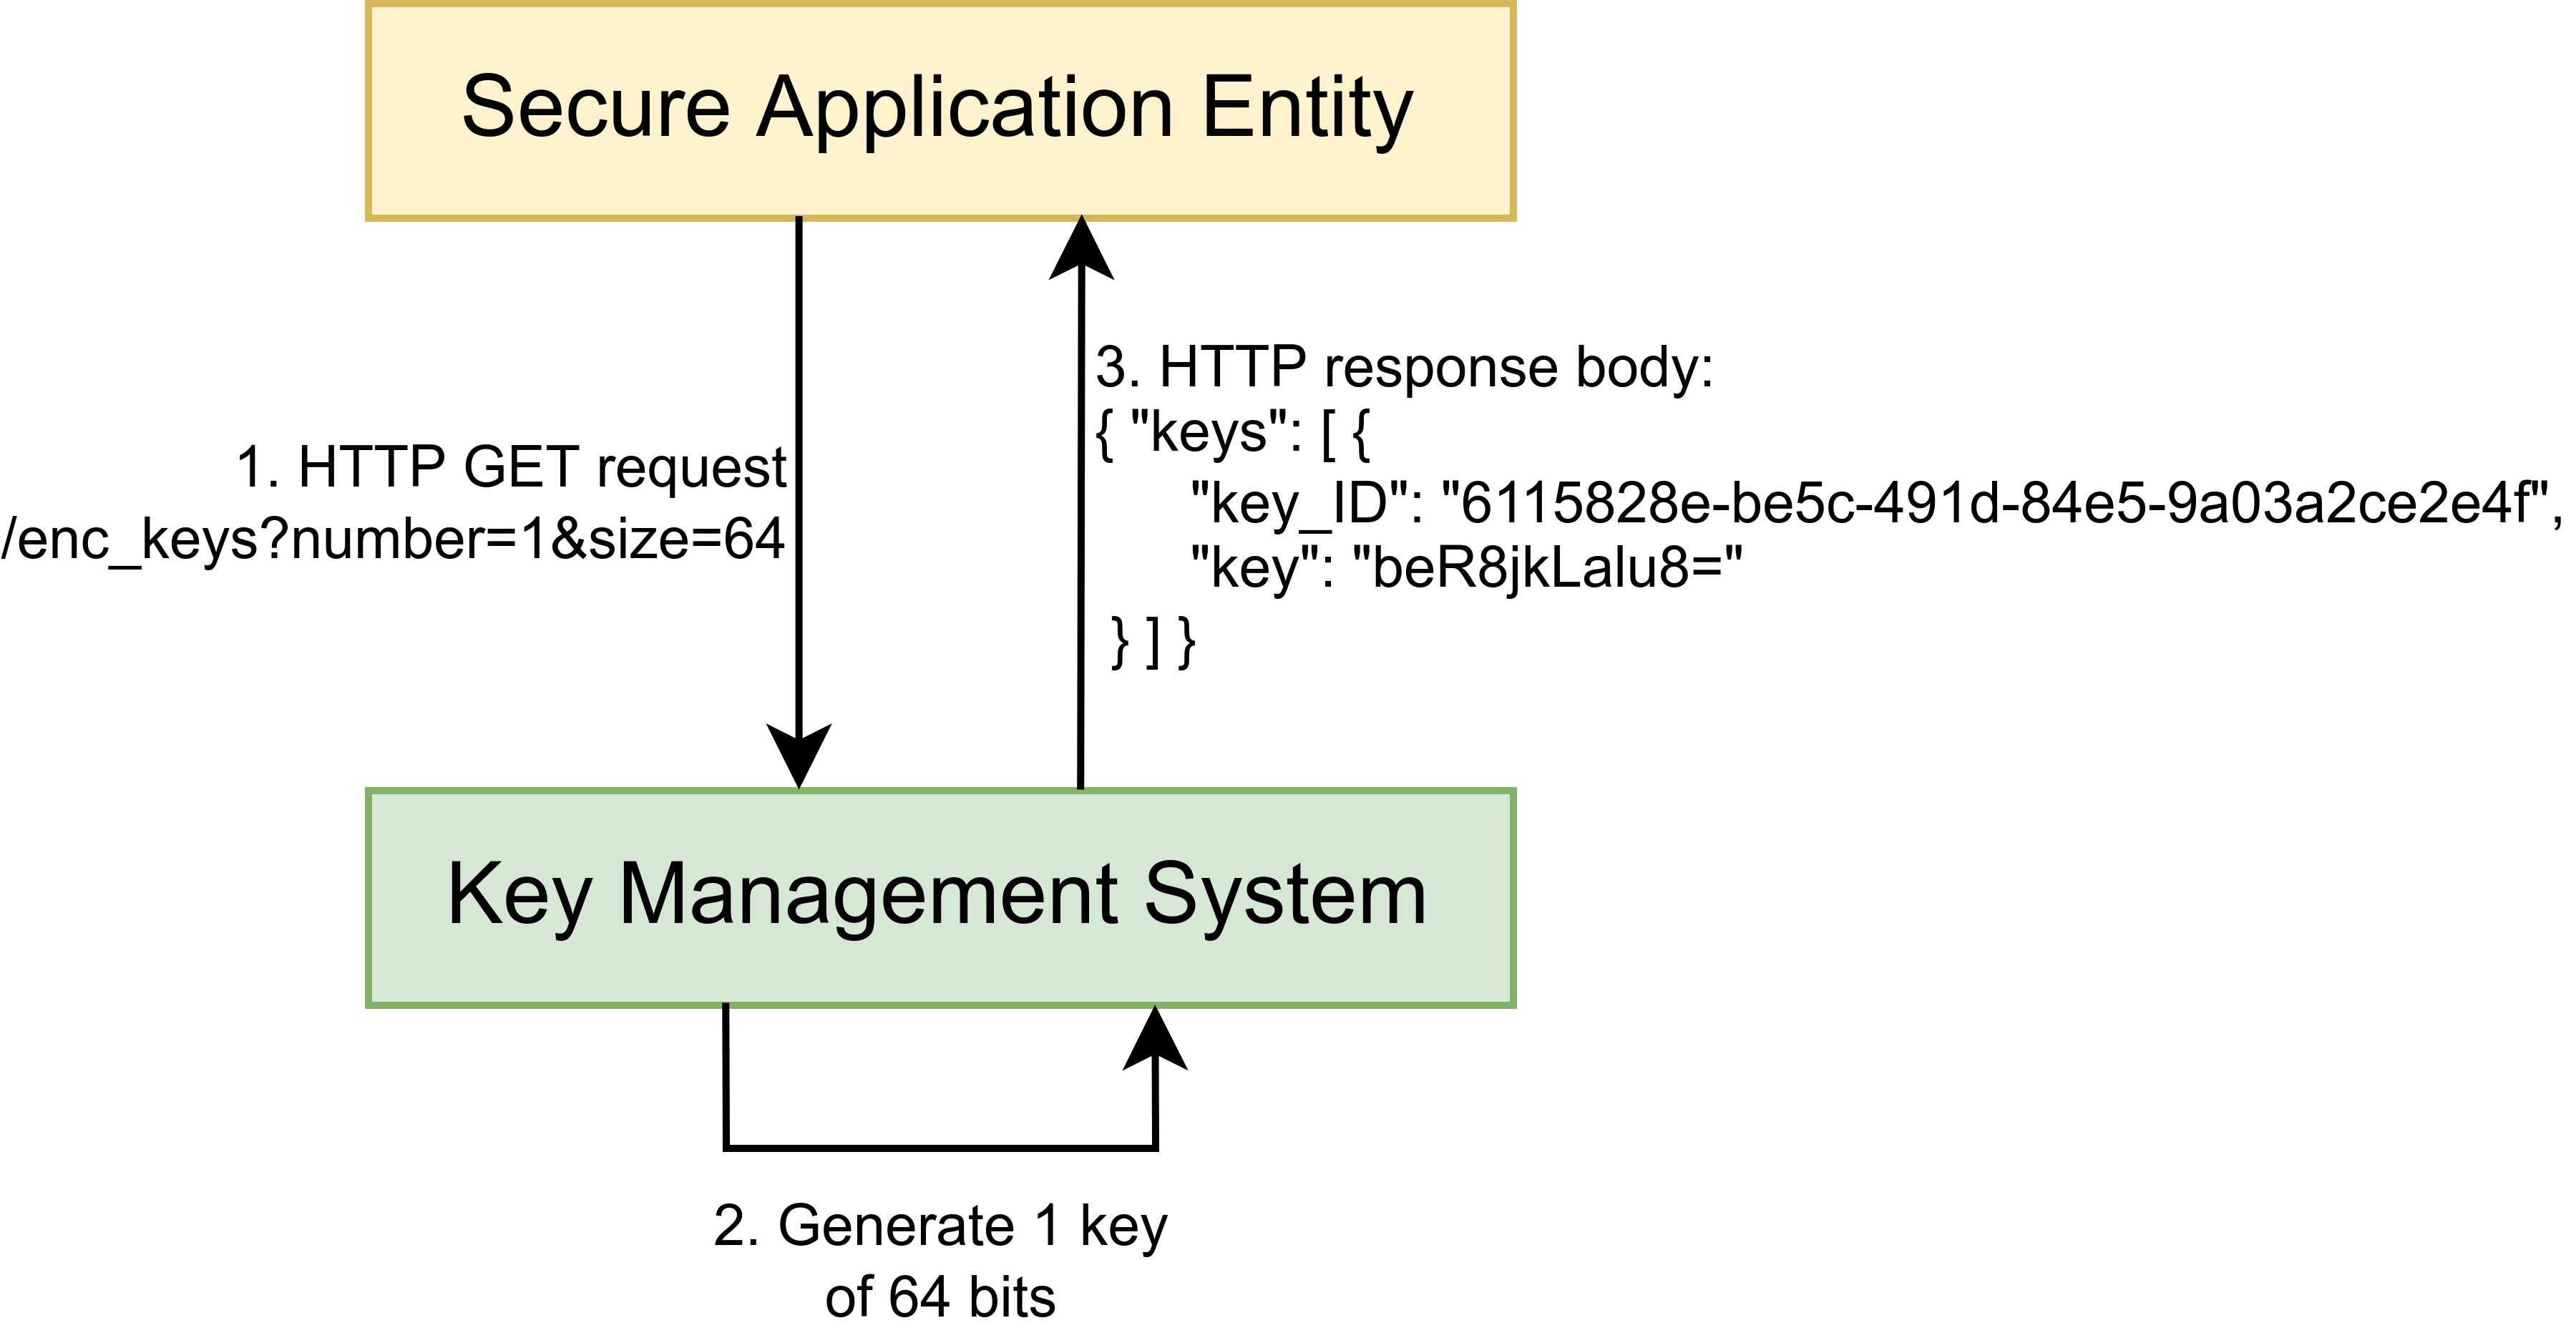
\includegraphics[width=0.8\textwidth]{Images/get_key.png}
    \caption{An example of a successful key generation request.}
    \label{fig:get_key}
\end{figure}

\subsection{Getting keys by ID}

\subsubsection{Keys by IDs request}
After one master SAE requests the generation of a new key, it communicates the UUID of that key to one or more slave SAEs. These can ask their KME to get the key material associated with a given key UUID.

A slave SAE that needs to retrieve the key associated with a given UUID can use the HTTP GET method \textit{/dec\_keys}, specifying the "key\_ID" as a request parameter.

For example, if a SAE wants to retrieve the key material associated to the key ID "ed4a8b14-0f5e-44c3-a28c-46e3df35dda4", it should send an HTTP GET request with the following path:
\mint{latex}{/dec_keys?key_ID=ed4a8b14-0f5e-44c3-a28c-46e3df35dda4}

Sometimes, one SAE may need to request the keys associated with multiple key IDs. In this case, the SAE may exploit the HTTP POST method \textit{/dec\_keys}. Instead of specifying the "key\_ID" parameter, the HTTP POST method has a body whose data format is defined as a Key IDs JSON data format. The Key IDs JSON data format looks like this:

\begin{minted}{json}
{
  "key_IDs": [
    { "key_ID": "ed4a8b14-0f5e-44c3-a28c-46e3df35dda4" },
    { "key_ID": "23e0dfa1-e6f8-4477-a2c8-c7b0f9684769" }
  ]
}
\end{minted}

\subsubsection{Keys by IDs response}
As shown in the figure above, a Key IDs JSON object is an array of key IDs. If the KME can retrieve the key of each key\_ID specified in the request body, the operation is considered successful. The HTTP response body will contain a Key Container JSON object with all the keys requested. More details about Key Containers are available in the previous section.

Otherwise, if one or more keys associated with the given UUIDs cannot be reconstructed, the HTTP response will report a failure. The HTTP protocol gives the response's status by the so-called "HTTP status code", an integer number of three digits. For example, a successful GET request has an HTTP status code of 200. A failure is usually reported with a status code starting with digit 4, such as "400". For more details about HTTP status codes, please see \cite{http_status_codes}.

The way the KME retrieves a key, given its UUID, is described in the following sections.

Here is an example overview of a successful key by ID request:

\begin{figure}[H]
    \centering
    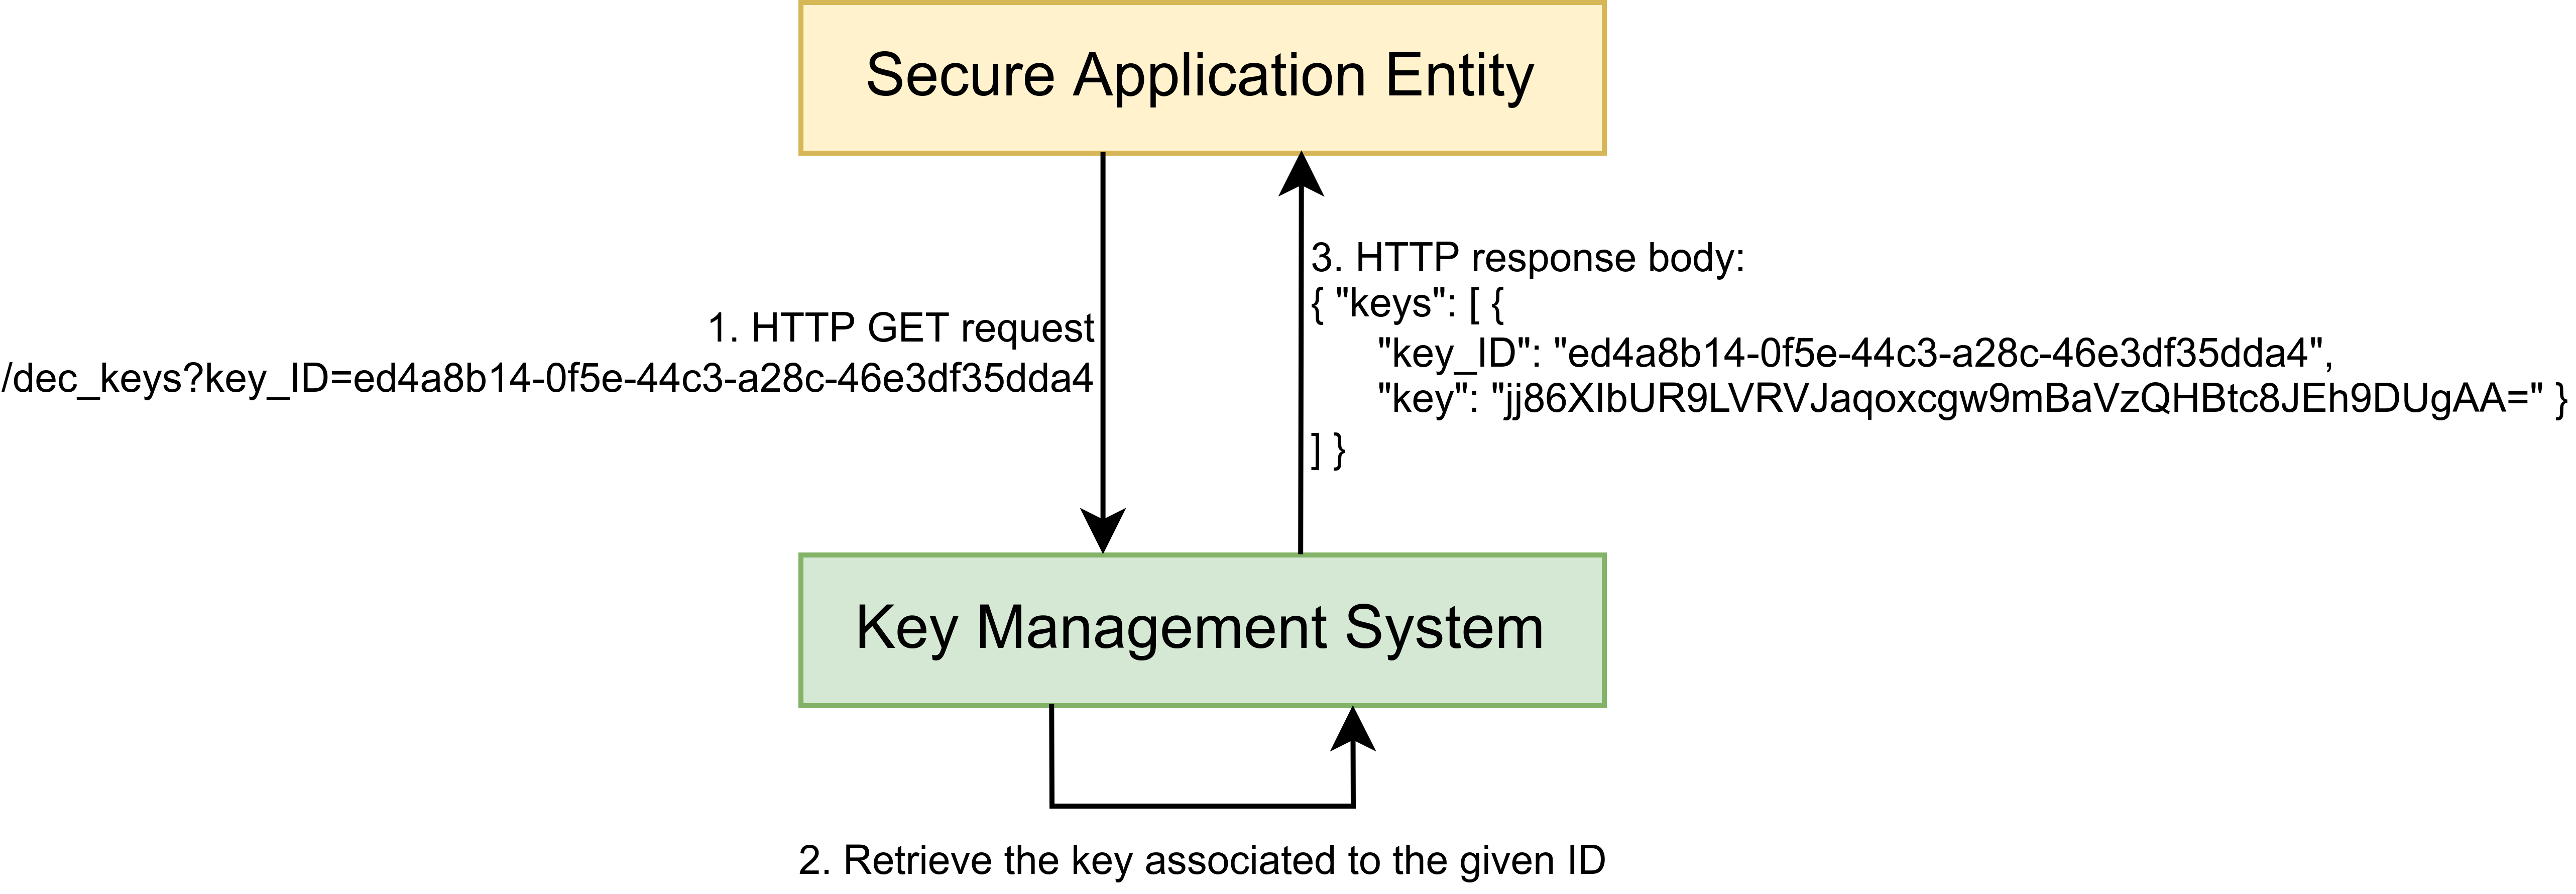
\includegraphics[width=1.0\textwidth]{Images/get_key_by_id.png}
    \caption{An example of a successful key by ID request.}
    \label{fig:get_key_by_id}
\end{figure}

\subsection{Requesting the status of the KME}
A Secure Application Entity may request the status of the Key Management Entity through the HTTP GET method available at path \textit{/status}.

When asked, the KME sends to SAE an HTTP response whose body contains a Status JSON object. The status JSON object includes some useful fields like:

\begin{itemize}
    \item key\_size: the default size, in bits, of key the KME can deliver to the SAE
    \item max\_key\_per\_request: the maximum number of keys a SAE may request with a single HTTP call
    \item max\_key\_size: the maximum size, in bits, of key the KME can deliver to the SAE
\end{itemize}

For a complete list of the fields inside a Status JSON object, please see page 14 of the standard mentioned above. 

\section{The interaction between the KME and the QC}
\label{kme:qc}

The previous section examined the interaction between KME and SAE, providing an overview of the standard ETSI GS QKD 014, exploited to implement the interface between the two entities mentioned above.

This section focuses on the interaction between the KME and a QKD Entity that is part of a Quantum Channel. For brevity, we often say: "The interaction between the KME and the Quantum Channel (QC)".

A Quantum Channel is a pair of devices that can securely exchange a secret sequence of bits, exploiting Quantum Key Distribution protocols. The product of a QKD exchange is called "block". Each block is identified by a UUID and contains the sequence of bits resulting from the key exchange. That sequence is called "block material".

The interface between the KME and the QC is not standardized. In particular, our implementation of this interface is based on conventions established in Politecnico di Milano.

When the Quantum Channel produces a new block, each QKD Entity of that channel sends the block to its KME. Therefore, the two KMEs involved will have a copy of the same block. In the following sections, we will see how a KME can produce keys starting from blocks and how it can communicate with the other KME to re-build that key.

Right now, we will specify how the QC sends blocks to KMEs.

The QKD Entity and the corresponding KME are linked through TCP socket connection \cite{socket}, a network-level API interface that allows two endpoints to communicate through a network. The API interface is simple: each KME is always listening on the socket connection, waiting for new blocks coming from the Quantum Channel.

When a QKD exchange is successful, each module of the Quantum Channel sends the very same block to the corresponding KME through the socket interface. In particular, the message is a JSON representation of the block. The Block JSON object has the following fields:

\begin{itemize}
    \item \textit{id}: the UUID of the block, chosen during the QKD exchange;
    \item \textit{key}: the block material, that is, the sequence of bits exchanged thanks to the QKD protocol. Notice that the block material is identified with the equivocal term "key" for compatibility reasons.
    \item \textit{time}: a timestamp identifying when the block has been produced;
    \item \textit{link\_id}: the UUID of the quantum channel that produced this block. Indeed, as it will be shown in \ref{ch4:exp3}, this implementation of the KME can receive and manage blocks coming from different quantum channels. The current chapter focuses on the interaction between the KME and only one Quantum Channel for clarity reasons.
\end{itemize}

When the KME receives a new block through the socket interface, it stores it locally. The block has to be stored confidentially not to break the security assumptions of the key management process. That block will then be used to build new keys or to re-build a key, given a key UUID.

\section{The internal functioning of the KME}
We analyzed how Secure Application Entities can request keys to Key Management Entities and how Quantum Channels can send blocks to KMEs. Now we are ready to dive into the internal functioning of the KME.

First, we will introduce two sub-sections of a KME devoted to storing blocks and instructions on how to re-build keys. Then, we will analyze the sequence of events that leads to the generation of a new key. In the end, we will focus on the process of retrieving keys, given their UUIDs.

\subsection{Local and shared storage}

\subsubsection{Storing blocks}
When the KME receives a newly-generated block from a Quantum Channel, it has to store it locally. This storage cannot be shared with anyone because it contains block material, the asset that has to be known only to the two collaborating KMEs.

In particular, a block stored in the local database contains the following pieces of information:

\begin{itemize}
    \item \textit{block\_id}: the UUID of the block;
    \item \textit{material}: the block material;
    \item \textit{timestamp}: the timestamp of the block;
    \item \textit{available\_bits}: an integer number that points out how many bits of the block were not exploited so far. When the block is inserted into the database, this field is equal to the length of the key material of the block. If, for example, the first ten bits of key material are exploited in order to build a key, the value of \textit{available\_bits} will be decreased by 10;
    \item \textit{link\_id}: the UUID of the quantum channel that produced this block.
\end{itemize}

Notice that, despite some changes in the name of the fields, \textit{available\_bits} is the only one added to the block by the KME when it has to store the block locally.

We will often refer to this local database as \textbf{local block DB}.

\subsubsection{Storing key instructions}
When the KME produces a new key, it has to store the instructions about how the key was built (i.e., which bits of which blocks were used to build the key material) in a database shared with the companion KME. The other KME will have to read those instructions to re-build the key. One KME cannot communicate the key material directly to the other KME: this would compromise the security assumptions of all the systems. The only communication of confidential bits between entities of the same kind is performed by the QKD Entities of the Quantum Channel, exploiting Quantum Key Distribution protocols.

The KME, after having created a key successfully, stores the instructions in the shared database. For each key, these pieces of information are stored:

\begin{itemize}
    \item \textit{key\_id}: the UUID of the key;
    \item \textit{instructions}: a list of instructions. Each instruction has the following structure:
    \begin{itemize}
        \item \textit{block\_id}: the UUID of the exploited block;
        \item \textit{start}: the index of the first bit of this block used in order to build the key material. Indexes start from 0 up to the length of the block material.
        \item \textit{end}: the index of the first bit of this block \textit{not} used in order to build the key material. It has to be a value greater than "start" and smaller or equal to the length of the block material. It is equal to the length of the block material only if the block material has been completely consumed.
    \end{itemize}
\end{itemize}

In our implementation of a KME, much care is taken to avoid repeated usage of the same bit to create two distinct keys.

The precise way instructions are created is described in the next section.

We will often refer to the shared database we have just described as \textbf{shared key DB}, or "shared DB".

\subsection{Generating new keys}
A master Secure Application Entity may request to the Key Management Entity the generation of new keys through the key delivery API implemented following the standard ETSI GS QKD 014, as seen in \ref{kme:key_gen}.

Now, we will describe how the KME manages the generation of N keys of size S.

The following procedure is repeated for each of the N keys requested:

\begin{enumerate}
    \item First, a new UUID is generated: it will be associated with the key after its material has been created.
    \item Then, construction of the key material begins. First, the KME picks up a block fragment from the local block DB. Then, it takes bits from the block material up to reaching the requested key length or up to finishing the bits of that block. Finally, the instruction pointing out the part of block material exploited is added to the list of instructions for that key.
    \item If the bits of the block material are exhausted and the requested key length is not reached, then the KME picks up another block from the local block DB and repeats the above process. 
    \item If the requested key length is reached, the KME stores the instructions for building that key in the shared database and proceeds to create the following key. Suppose the requested key length is reached, but the currently-exploited block has bits remaining. In that case, the block is re-inserted into the local block DB, coherently updating the value of its field \textit{available\_bits}.
    \item If all the N requested keys are generated, the KME returns them to the calling SAE through an HTTP response with status code 200, whose body is a Key Container that includes such keys. For more details about the structure of a Key Container, see \ref{kme:key_container}.
    \item If the KME does not find any available block fragment or in case of any other possible error, an HTTP response with status code 400 is returned. For more details about the status codes returned by the KME in case of errors, please refer to the standard ETSI GS QKD 014.
\end{enumerate}

The following figure shows the sequence of events that starts with a key generation request by a SAE and ends with the HTTP response given by the KME, containing the requested number of keys.

\begin{figure}[H]
    \centering
    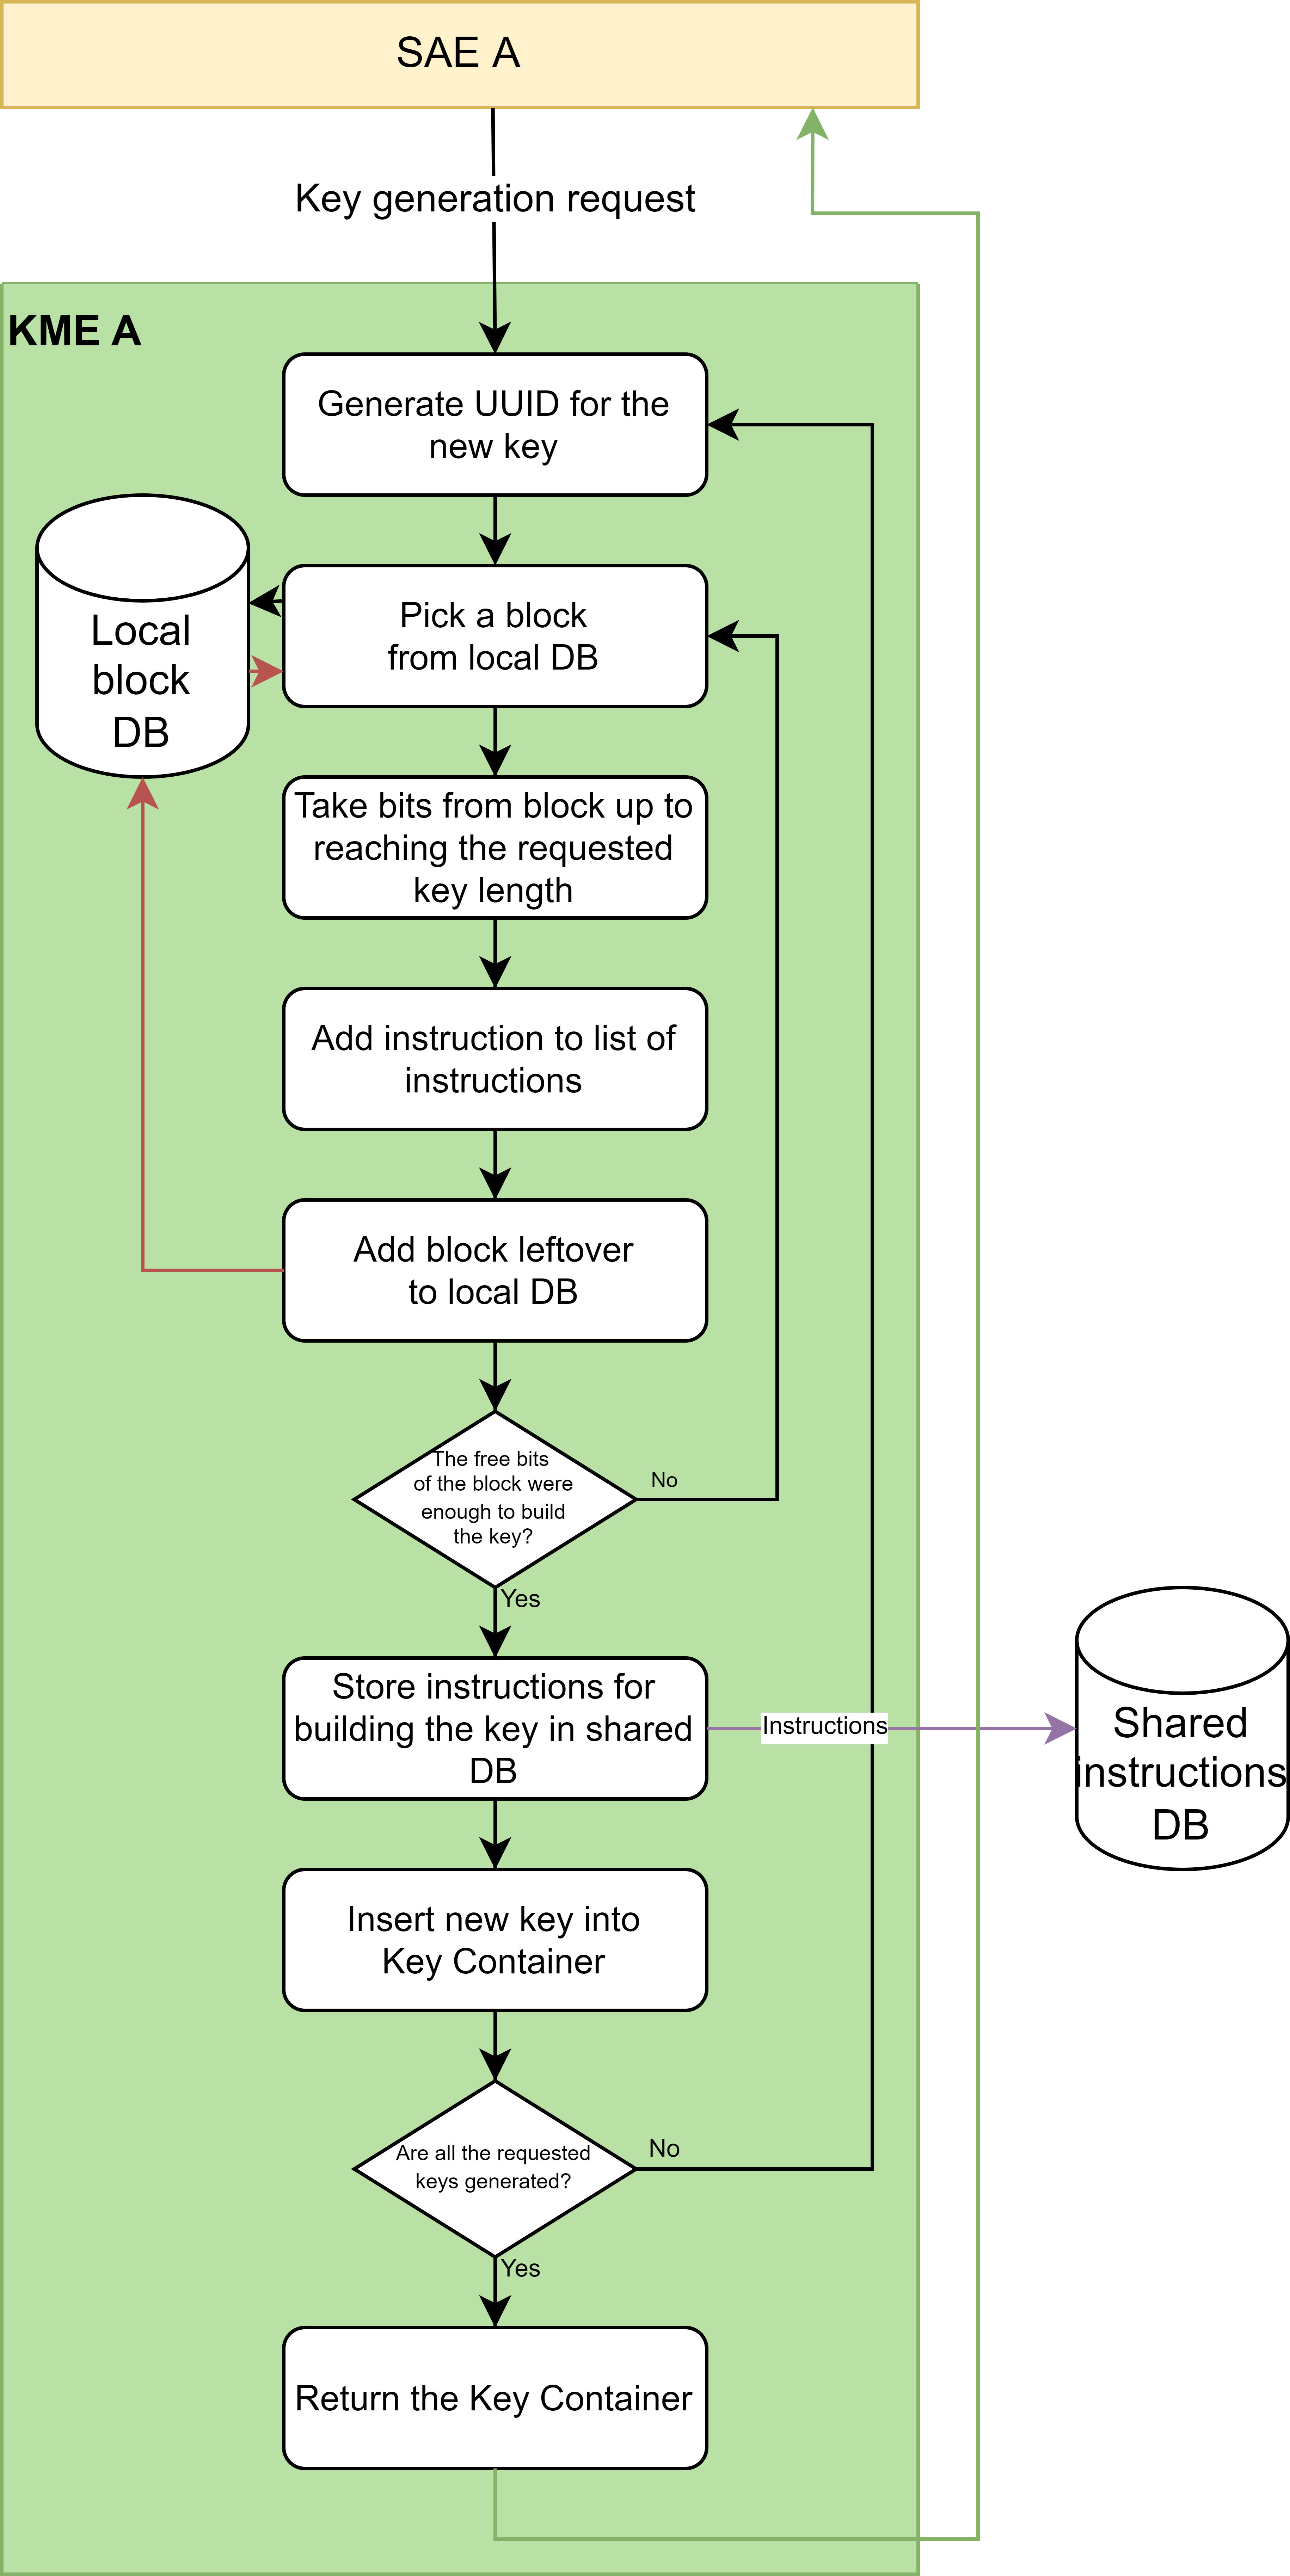
\includegraphics{Images/key_generation.png}
    \caption{The management of a key generation request.}
    \label{fig:key_generation}
\end{figure}

\subsection{Getting blocks by ID}
After one master SAE requested the generation of N keys of length S to one KME, other slave SAEs may request to retrieve those keys to the other KME. In this paragraph, we describe the process of retrieving keys, given their UUIDs, step by step.

When KME receives a request for getting keys associated with given UUIDs, for each UUID:

\begin{enumerate}
    \item First, it reads from the shared DB the instructions associated with the given UUID. If no instructions are associated with the UUID, the KME returns an HTTP response with status code 404.
    \item If there are instructions associated with the given key UUID, then the KME reads them. Each instruction contains the UUID of a block. Then, the KME retrieves that block from the local DB. Again, suppose there is no block associated with the given UUID. In that case, the KME returns an HTTP response with a failure status code.
    \item For each block retrieved, the KME extracts the bits pointed out in the corresponding instruction. This process allows to re-build the key material of the key with the given UUID.
    \item If a key is correctly re-built, it is inserted into the Key Container that will be the body of the HTTP response.
    \item If all the requested keys have been correctly re-built, the KME returns an HTTP response with status code 200, whose body is the Key Container that includes the keys re-built starting from their UUIDs.
\end{enumerate}

The following figure shows the sequence of events that starts with a key retrieval request by a SAE and ends with the HTTP response given by the KME, containing the requested keys. For simplicity and readability, it shows the path followed in case of a successful request.

\begin{figure}[H]
    \centering
    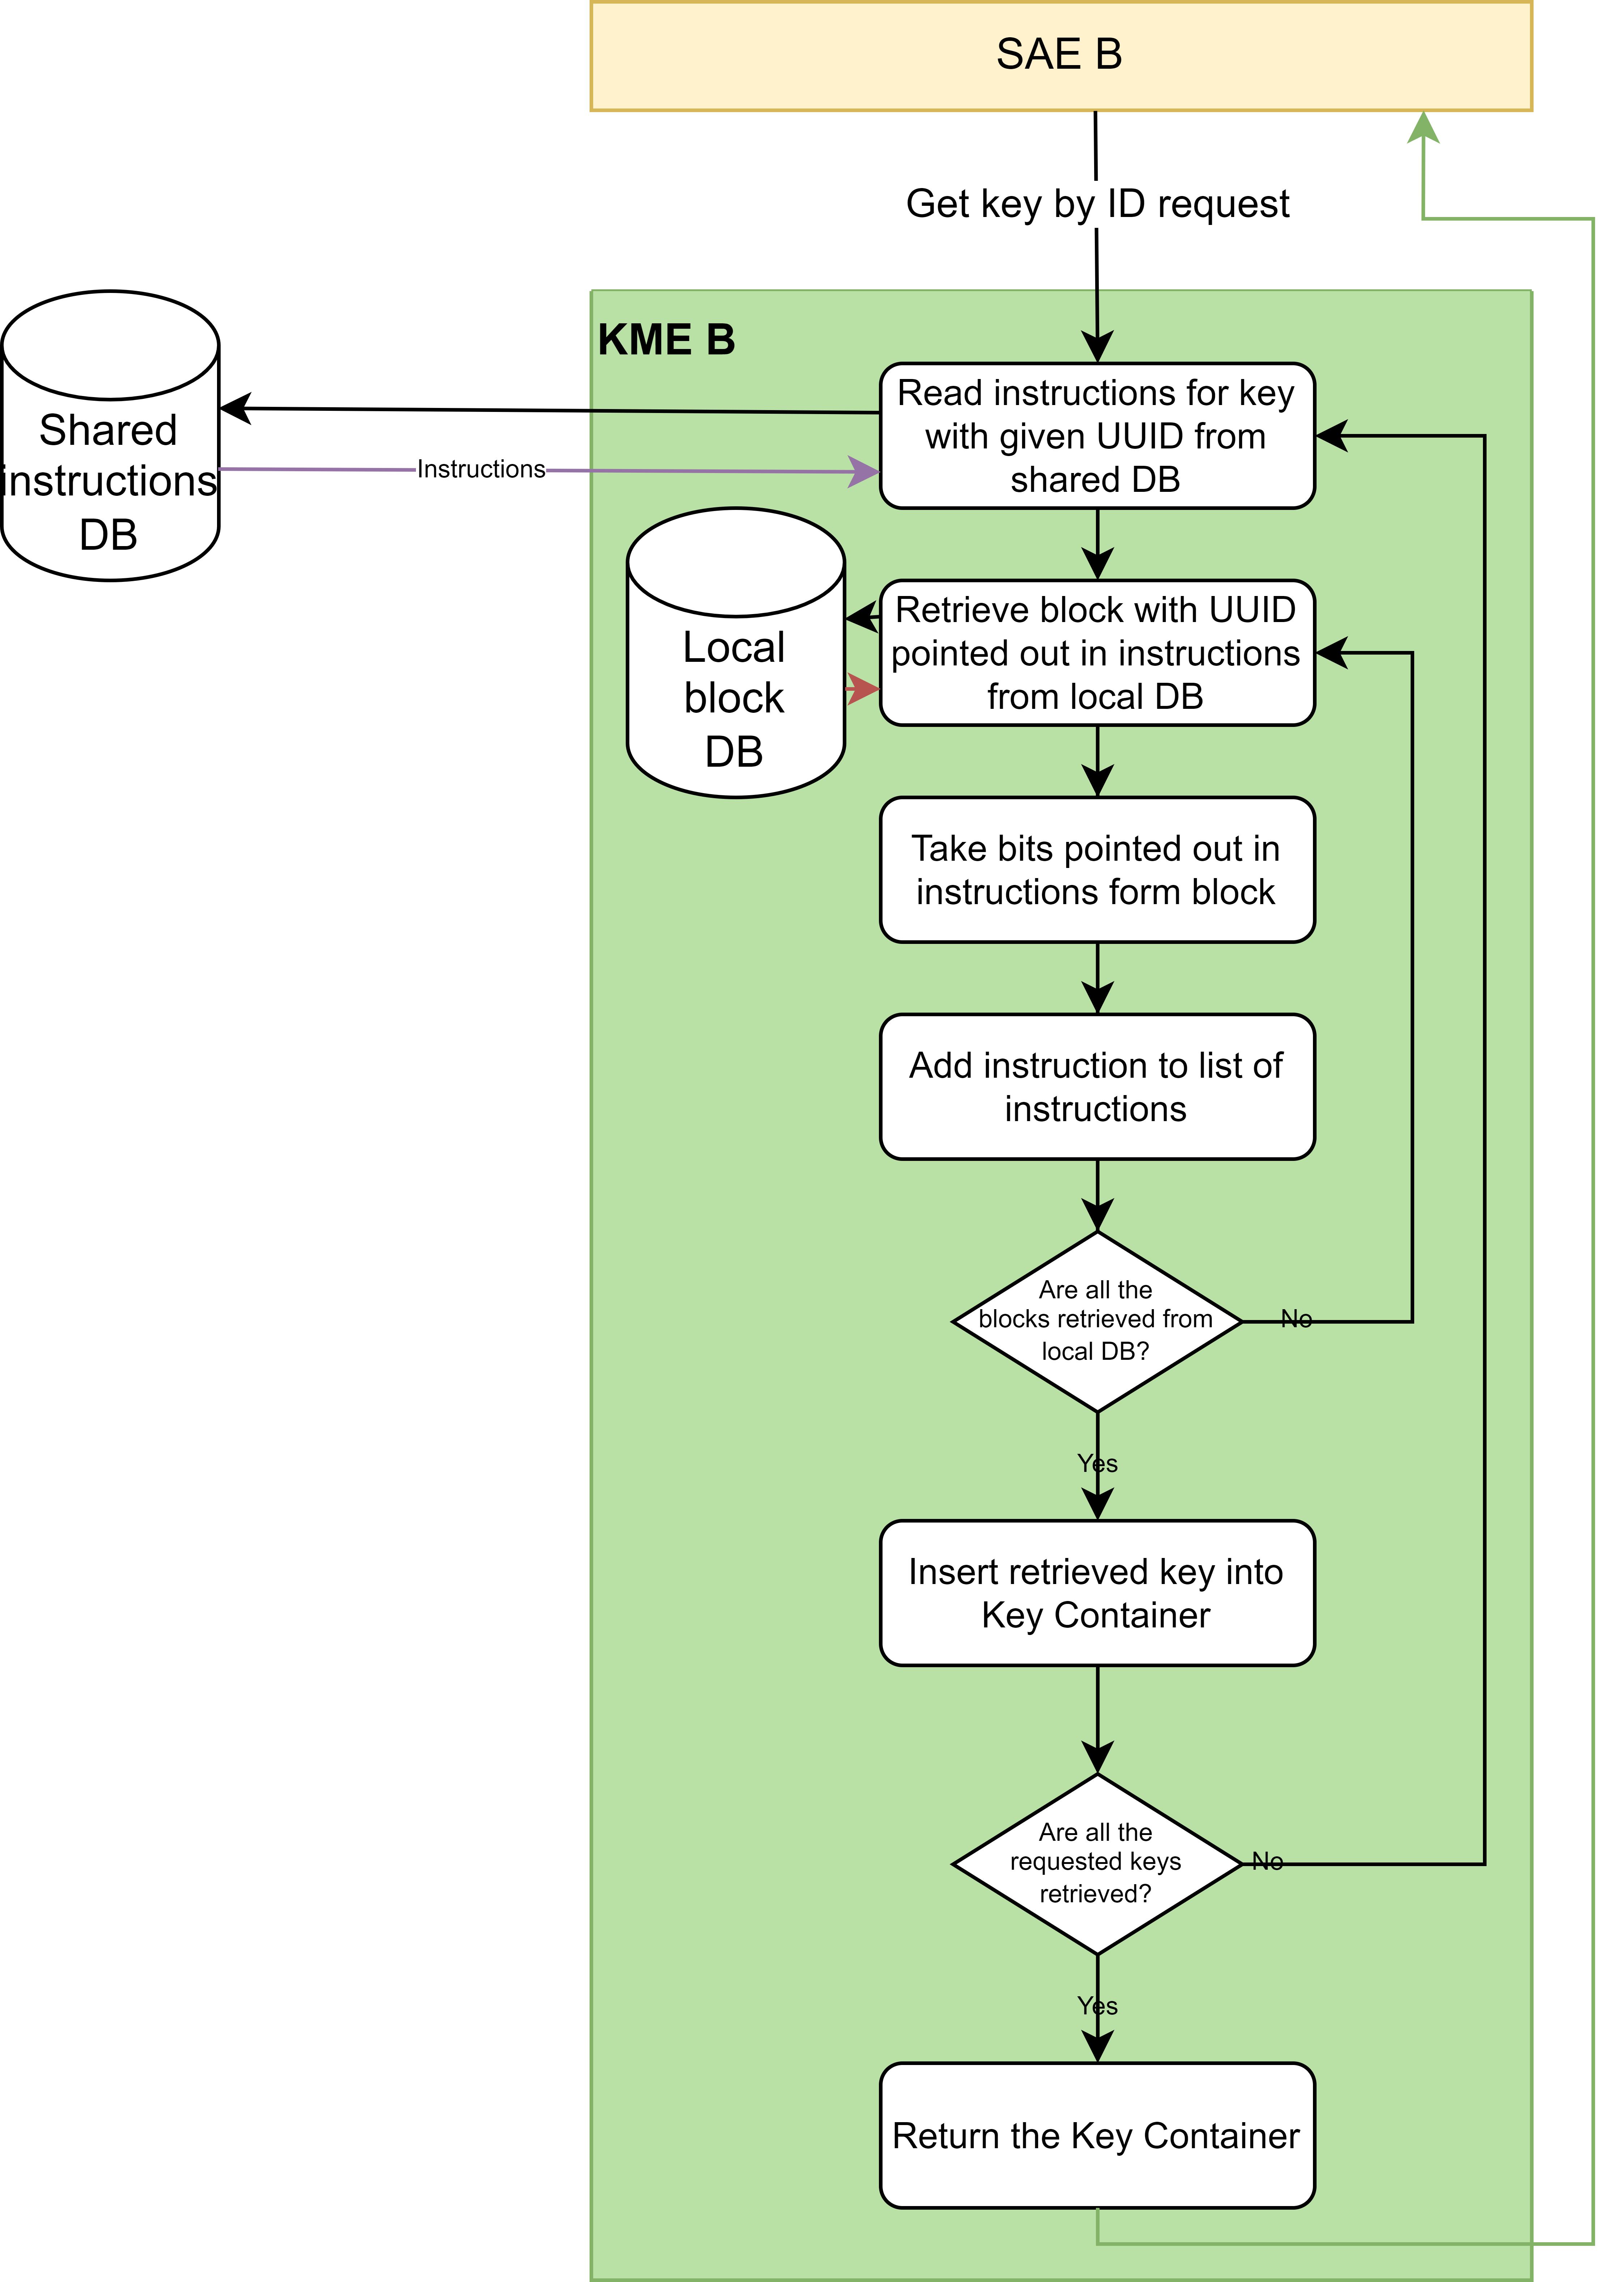
\includegraphics{Images/key_retrieval.png}
    \caption{The management of a key retrieval request.}
    \label{fig:key_retrieval}
\end{figure}

\subsection{The cooperation between KMEs}
At the end of this chapter, we can have a complete overview of the key management process.
It all starts with the request to generate one or more keys by a Master SAE to its KME through the API described in the ETSI standard. We refer to the Master SAE as "SAE A" and its KME as "KME A".
SAE A communicates the UUIDs of the keys received from KME A to other SAEs. We refer to them as "SAE B". SAE B is a Slave SAE, which requests from its KME - "KME B" - the keys associated with the UUIDs received from SAE A.
Finally, thanks to this process, the SAEs have the same keys, which have been generated and distributed confidentially, to be used, for example, for encrypting future communications.

The following figure summarizes the entire process of key distribution made possible thanks to Key Management Entities. We used the ID "abc" for the requested key for simplicity and readability. However, keep in mind that a UUID identifies the keys.

\begin{figure}[H]
    \centering
    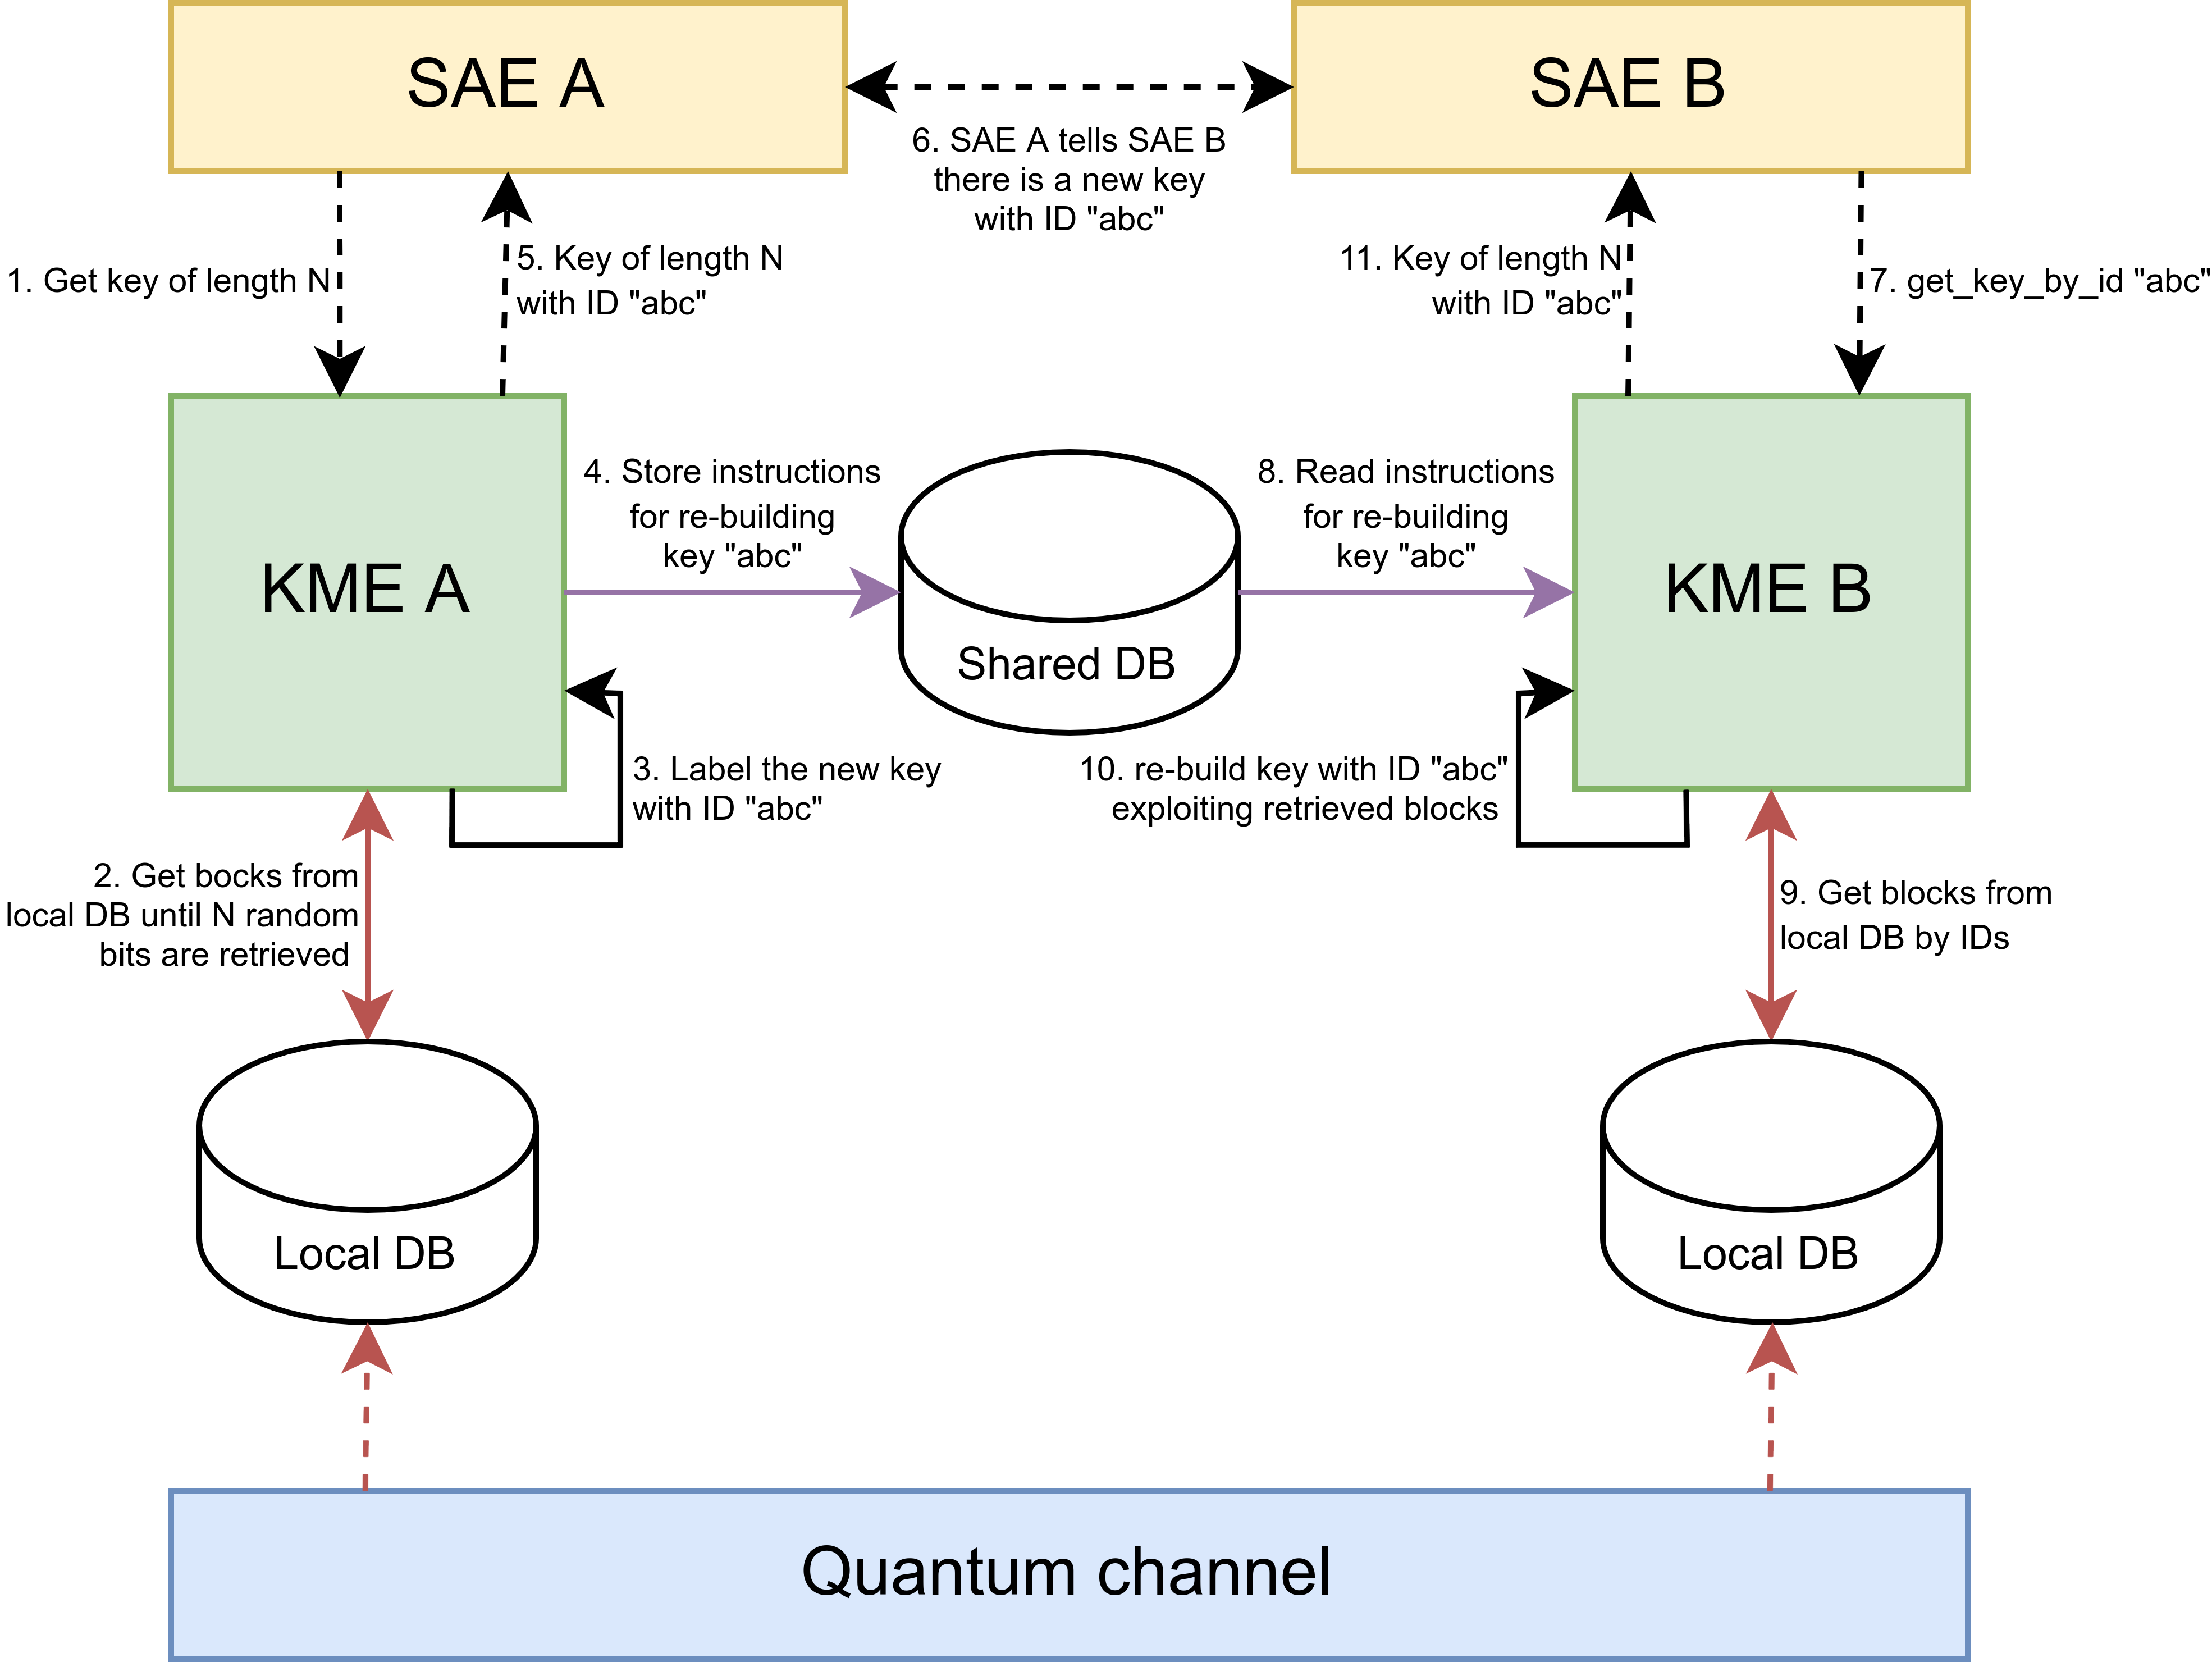
\includegraphics[width=1.0\textwidth]{Images/sequence_diagram.png}
    \caption{A complete overview of the key management process.}
    \label{fig:sequence_diagram}
\end{figure}
